\documentclass{standalone}
\usepackage{tikz}
\usetikzlibrary{calc}
\usetikzlibrary{decorations.pathreplacing,calligraphy}
\usepackage{pgfplots}
\usetikzlibrary{intersections, pgfplots.fillbetween}
\usetikzlibrary{snakes}
\usepackage{xcolor}

\begin{document}

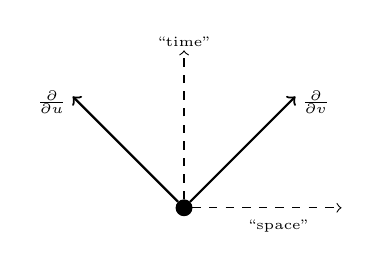
\begin{tikzpicture}[scale=1]

\node[circle, draw, fill, inner sep =0, minimum size = .2cm] (n1) at (0,0) {};

\draw[->, dashed] (n1) -- (0,2);
\draw[->, dashed] (n1) -- (2,0);
\draw[->, thick] (n1) -- (135:2);
\draw[->, thick] (n1) -- (45:2);

\node[label = below:\tiny``space"] at (1.2,.1) {};
\node[label = above:\tiny``time"] at (0,1.8) {};
\node[label = left:\tiny $\frac{\partial}{\partial u}$] at ($(135:1.9)+(0:.1)$) {};
\node[label = right:\tiny $\frac{\partial}{\partial v}$] at ($(45:1.9)+(0:-.1)$) {};


\end{tikzpicture}


\end{document}